\section{Le 3b-1}

% \subsection*{(a)}
% The code and figure generating 500 particles to represent the distribution with equal weight is as follows:
% \begin{matlabcode}
% N = 500;
% w = 1/N + zeros(1,N);
% for ii = 1:N
%     x(ii) = normrnd(0,1) * w(ii);
% end
% [fx,xk]=ksdensity(x); 
% \end{matlabcode}
The Sample generated by 500 particles to represent the distribution with equal weight is as follows:
\begin{figure}[!h]
    \centering
    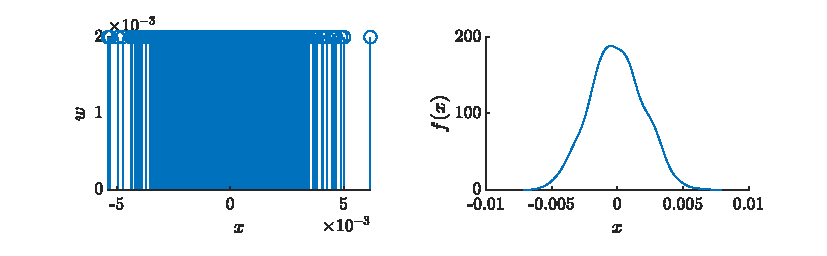
\includegraphics{figures/ex4_a.pdf}
\end{figure}

\newpage 
The particles from the exercise were used to compute new particles such that the new particles represent the distribution with the following relation:
\begin{align*}
    y = \sin(2\pi x^2),
\end{align*}
representing the distribution is shown in the figure below:
\begin{figure}[!h]
    \centering
    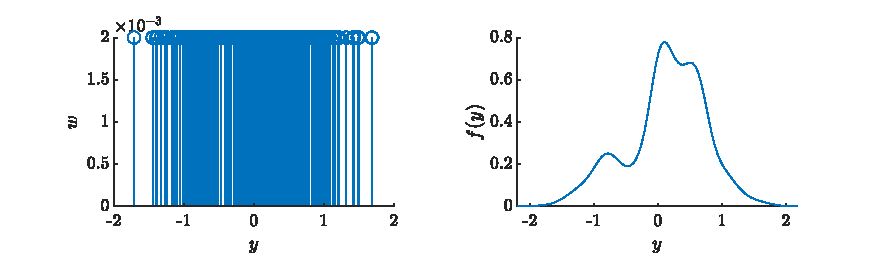
\includegraphics{figures/ex4_b.pdf}
\end{figure}
